\documentclass[13pt,a4paper]{article}
\usepackage{amsmath}
\usepackage[utf8]{vietnam}
\usepackage{amsfonts}
\usepackage{amssymb}
\usepackage{graphicx}
\usepackage{float}
\usepackage{multicol}
\usepackage{tkz-tab}
\usepackage{colortbl}
\usepackage{multicol}
\usepackage[left=2cm,right=2cm,top=2cm,bottom=2cm]{geometry}
\setlength{\parindent}{0pt}
\begin{document}
\fontsize{18}{30}\selectfont
{\centering TRƯỜNG ĐẠI HỌC CÔNG NGHỆ THÔNG TIN \\
KHOA KHOA HỌC MÁY TÍNH \\
\par}
\vspace{0.5 cm}
\begin{center}
    \begin{figure}[htp]
     \centering
\includegraphics[scale=.3]{images/logo_uit.jpg} \\
    \end{figure}
    \vspace{1 cm}
    
    \par\noindent\rule{\textwidth}{0.5pt}
    \fontsize{14}{30}\selectfont
    {\centering \textbf{Assignment 1 \\
     DFS/BFS/UCS for Sokoban \\
    }
    \par\noindent\rule{\textwidth}{0.5pt}
    
    \fontsize{14}{30}\selectfont
    \begin{tabbing}
    \hspace{2 in} \= \hspace{2 in} \= \kill
    Môn: \> Trí tuệ nhân tạo \\
    Lớp: \> CS106.N21.KHCL \\
    Giảng viên hướng dẫn: \> Lương Ngọc Hoàng \\
    Sinh viên: \>Bùi Mạnh Hùng - 21522110 \\
    \end{tabbing} 
    \date{\today}
    \begin{center}
          \vfill
          \today 
    \end{center}
\end{center}
\newpage

\begin{document}
\tableofcontents
\clearpage
\fontsize{13}{14}\selectfont
\section{Bài toán Sokoban}
\subsection{Mô hình hóa Sokoban}
\textit{\textbf{Sokoban được mô hình hóa dưới dạng bài toán tìm kiếm trạng thái}}
\subsubsection{Tài nguyên}
Có 18 levels nằm trong thư mục "../assets/sokobanLevels", biểu diễn dưới dạng file .txt
\begin{figure}[H]
    \centering
    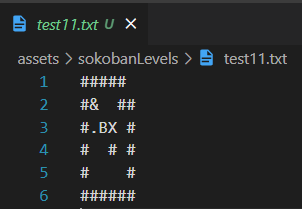
\includegraphics[scale=1.2]{images/txt11.png}
    \caption{Map of level 11}
\end{figure}
\textbf{Chú thích}
\begin{multicols}{2}
\begin{itemize}
    \item ' ': Free space
    \item '\#': Wall
    \item '\&': Player
    \item 'B': Box
    \item '.': Goal
    \item 'X': Box on goal
\end{itemize}
\end{multicols}
\subsubsection{File Level.py}
Dùng để convert những ký tự chữ trong trong file .txt(Hình 1) thành những ký tự số được định nghĩa trong file constants.py
\begin{figure}[H]
    \centering
    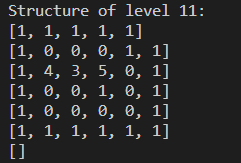
\includegraphics[scale=1.5]{images/structureLevel11.png}
    \caption{Structure of level 11}
    \label{fig:my_label}
\end{figure}
\textbf{Chú thích}
\begin{multicols}{2}
\begin{itemize}
    \item 0 : AIR(Free space)
    \item 1 : WALL
    \item 2 : PLAYER
    \item 3 : BOX
    \item 4 : TARGET(Goal)
    \item 5 : TARGET\_FILLED(Box on goal)
\end{itemize}
\end{multicols}
\subsubsection{Function 'transferToGameState2()'}
\textbf{Input:}
\begin{itemize}
    \item layout: Lấy từ structure của file level.py
    \item player\_pos: Lấy từ position\_player của file level.py 
\end{itemize}
\textbf{Output:} gameState kiểu numpy.ndarray bao gồm layout và vị trí người chơi

\subsubsection{Function 'get\_move()'}
\textbf{Input:}
\begin{itemize}
    \item layout: Lấy từ structure của file level.py
    \item player\_pos: Lấy từ position\_player của file level.py 
    \item method: Thuật toán tìm kiếm (dfs/bfs/ucs/..)
\end{itemize}
\textbf{Output:} Result \& runtime

\subsubsection{Function 'auto\_move()'}
\begin{itemize}
    \item Lựa chọn thuật toán tìm kiếm để thực thi
    \item Lưu kết quả chạy vào file .txt
\end{itemize}
\subsection{Trạng thái khởi đầu \& kết thúc}
\subsubsection{Trạng thái khởi đầu}
Trạng thái khởi đầu được load lên từ Class Level bao gồm list dữ liệu được trích từ các file .txt tương ứng với mỗi level. => Sau đó nạp vào hàm transferToGameState2() trả về gameState \\
\textbf{Lưu trữ vị trí}\\
Hai biến global posWalls \& posGoals: Cố định trong thời gian thực thi
\begin{itemize}
    \item posWalls: giá trị trả về của hàm PosofWalls() có kiểu dữ liệu tuple lưu vị trí của các WALL trong game
    \item posGoals: giá trị trả về của hàm PosOfGoals() có kiểu dữ liệu tuple lưu vị trí của các GOAL trong game
\end{itemize}
Hai biến local beginBox \& beginPlayer: Thay đổi trong thời gian thực thi
\begin{itemize}
    \item beginBox: giá trị trả về của hàm PosOfBoxes có kiểu dữ liệu tuple lưu vị trí của các BOX trong game
    \item beginPlayer: giá trị trả về của hàm PosOfPlayer có kiểu dữ liệu tuple lưu vị trí của Player trong game
\end{itemize}
\subsubsection{Trạng thái kết thúc}
Hàm isEndState(): kiểm tra vị trị các BOX đã trùng với vị trí các GOAL hay chưa ? \\
=> Sắp xếp các vector của tập posBox và posGoals rồi so sánh với nhau\\
\subsection{Không gian trạng thái}
Hàm legalActions: quản lý không gian trạng thái, player có 4 hướng di chuyển:
\begin{figure}[H]
    \centering
    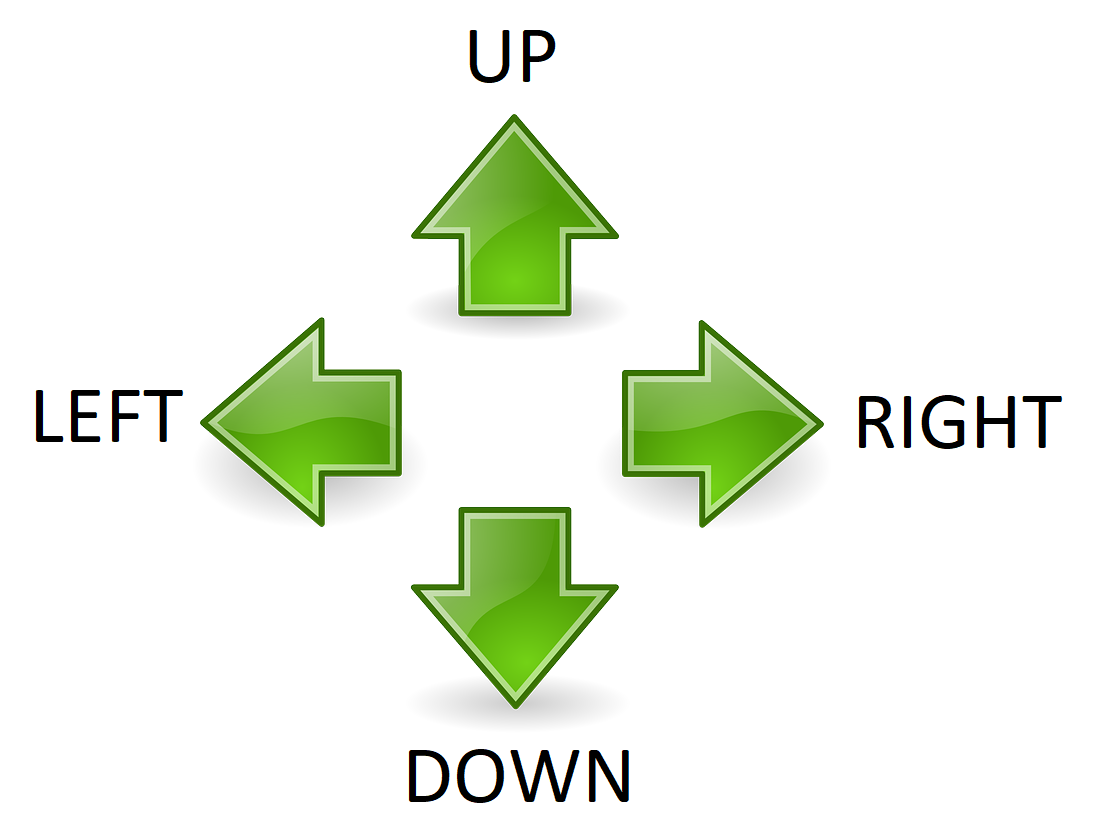
\includegraphics[scale=0.25]{images/udlr.png}
    \caption{4 directions}
    \label{fig:my_label}
\end{figure}
Danh sách các hành động có thể thực hiện của Player được lưu trữ trong list allActions[] theo dạng [x,y,a,A], trong đó:
\begin{itemize}
    \item x,y: offset so với vị trí hiện tại, có 4 kiểu \{(-1,0) , (1,0) , (0,-1) , (0,1)\}
    \item a,A: Hướng đi của player a\in {u,d,l,r} \& A\in{U,D,L,R} 
    \begin{itemize}
        \item a: di chuyển bình thường qua vị trí 'Free Space'
        \item A: di chuyển vào vị trí Box và đẩy Box theo hướng di chuyển 1 offset
    \end{itemize}
\end{itemize}
\fontsize{13}{15}\selectfont
Lặp các action trong list AllActions với vị trí tương ứng (xPlayer + action[0] , yPlayer + action[1]) với (xPlayer , yPlayer) là vị trí hiện tại \\
=> Kiểm tra tính hợp lệ của action trong hàm isLegalAction(), dựa vào kết quả trả về để thêm/không thêm action vào list legalActions[ ] \\
Sau đó, hàm legalActions() trả về tập các action hợp lệ.
\subsection{Các hành động hợp lệ}
Các hành động hợp lệ được xác định bởi hàm isLegalActions()\\
Vị trí xét (xPlayer + x,yPlayer + y) trong đó (xPlayer,yPlayer) là vị trí Player hiện tại;(x,y) offset của action đang xét 
Hành động được gọi là hợp lệ khi vị trí action không đi vào tường hoặc ở trong tường hay \textit{"pos\_action not in posBox + posWalls"}
\subsection{Hàm tiến triển(successor function)}
Successor function là hàm đánh giá ước lượng chi phí còn lại để đạt được trạng thái đích từ trạng thái hiện tại. 
\subsubsection{Đối với Depth First Search \&Breadth First Search Algorithm}
Hai thuật toán tìm kiếm này hàm tiến triển không được sử dụng vì chúng không cần đánh giá ước lượng chi phí còn lại. DFS, BFS tìm kiếm đường đi từ trạng thái khởi đầu đến trạng thái đích bằng cách duyệt qua tất cả trạng thái có thể đạt được từ trạng thái khởi đầu. \\
\subsubsection{Đối với Uniform Cort Search Algorithm}
Hàm tiến triển giúp tối ưu hóa việc tìm kiếm đường đi bằng cách cập nhật độ ưu tiên của các trạng thái dựa trên tổng chi phí đường đi đã đi qua và ước lượng chi phí còn lại đến trạng thái đích.\\
Hàm cost trong UCS: tổng quãng đường (số action thực hiện) trong actions(đi không đẩy thùng)
\section{Thống kê}
Số liệu thống kê các bước thực hiện, runtime: được lưu tại ../sokobanSolver/.. \\

\begin{table}[H]
    \fontsize{14}{20}\selectfont
        \centering
        \begin{tabular}[c]{|p{4cm}|p{.75cm}|p{.75cm}|p{.75cm}|p{.75cm}|p{.75cm}|p{.75cm}|p{.75cm}|p{.75cm}|p{.75cm}|p{.75cm}|}\hline
        Level & 1 & 2 & 3 & 4 & 5 & 6 & 7 & 8 & 9 \\ \hline
        DFS& 79 & 24 & 403 & 27 & X & 55 & 707 & 323 & 74 \\\hline
        BFS & 12 & 9 & 15 & 7 & 20 & 19 & 21 & 97 & 8 \\\hline
        UCS & 12 & 9 & 15 & 7 & 20 & 19 & 21 & 97 & 8 \\\hline
        \end{tabular}
        \caption{Số bước chạy của các thuật toán với Level: 1->9}
\end{table}
\begin{table}[H]
        \fontsize{14}{20}\selectfont
        \centering
        \begin{tabular}[c]{|p{4cm}|p{.75cm}|p{.75cm}|p{.75cm}|p{.75cm}|p{.75cm}|p{.75cm}|p{.75cm}|p{.75cm}|p{.75cm}|p{.75cm}|}\hline
        Level & 10 & 11 & 12 & 13 & 14 & 15 & 16 & 17 & 18\\\hline
        DFS& 37 & 36 & 109 & 185 & 865 & 291 & X & X & X \\\hline
        BFS & 33& 34 & 23 & 31 & 23 & 105 & 34 & X & X \tabularnewline\hline
        UCS & 33 & 34 & 23 & 31 & 23 & 105 & 34 & X & X \\\hline
        \end{tabular}
        \caption{Số bước chạy của các thuật toán với Level: 10->18}
\end{table}
\textit{\textbf{Chú thích: }}\\ X: Thuật toán không tìm ra đường đi
\section{Nhận xét}
Trong game Sokoban, chi phí cho mỗi action đều bằng 1 \\
\textbf{Lời giải của các thuật toán}\\ \\
\textit{Đối với thuật toán Depth First Search} \\
Kết quả thuật toán chưa tối ưu vì DFS tìm kiếm theo độ sâu và dừng lại khi tìm được một lời giải của bài toán nên có thể bỏ qua lời giải tối ưu ở các nhánh khác \\ \\
\textit{Đối với thuật toán Breadth First Search} \\
Kết quả thuật toán là tối ưu vì BFS đảm bảo tìm được đường đi ngắn nhất nếu tồn tại đường đi từ trạng thái hiện tại đến trạng thái đích. Tuy nhiên, thuật toán này có thể tốn nhiều bộ nhớ để lưu trữ tất cả các trạng thái đã duyệt qua. \\ \\
\textit{Đối với thuật toán Uniform Cost Search} \\
Kết quả thuật toán là tối ưu vì nó đảm bảo tìm được đường đi ngắn nhất từ vị trí hiện tại đến vị trí đích nếu tồn tại đường đi. Tuy nhiên trong trò chơi Sokoban, UCS có thể gặp vấn đề độ phức tạp tính toán và thời gian thực thi. \\ \\
\textbf{Thuật toán tối ưu nhất } \\
Việc đánh giá thuật toán nào tốt hơn mang tính khách quan vì phụ thuộc vào nhiều yếu tố: thời gian thực thi, không gian lưu trữ ,...Nhưng xét trong phạm vi trò chơi Sokoban với 18 levels và chi phí mỗi action đều bằng 1 thì BFS(Breadth First Search) sẽ tối ưu hơn so với UCS(Uniform Cost Search) vì:
\begin{itemize}
    \item Số lượng node được push vào hàng đợi PriorityQueue(UCS) = Queue(BFS)
    \item Độ phức tạp:
    \begin{itemize}
        \item BFS: O((E+V)logV)
        \item UCS: O(E+V)
    \end{itemize}
    Với V là số đỉnh, E là số cạnh của đồ thị.
\end{itemize}
\textbf{Các bản đồ của bài toán} \\
-Map 17,18,19 không có kết quả dù thử cả 3 thuật toán BFS,DFS,UCS\\
-Map 5,16 thì thuật toán DFS thực hiện quá lâu, nguyên nhân do:
\begin{itemize}
    \item Bản đồ lớn và số lượng ô trống nhiều dẫn đến cây tìm kiếm có nhiều trạng thái.
    \item Thuật toán DFS tìm kiếm theo độ sâu và duyệt hết lần lượt tất cả các nhánh.
\end{itemize}
\end{document}
